% Flight / Stay — ATP 2026 DCT Abu Dhabi proposal (v2: simplified technical English)
% Compile from this directory: tectonic flight_proposal_v2.tex
% v1 is flight_stay_proposal.tex/.pdf and is unchanged.
% Change the team fields below before submission.
% Visual system adapted from the supplied Design Report reference: white
% canvas, black sans-serif headings, generous margins, image-led cover,
% fine rules, restrained warm accent and quiet running footer.
\documentclass[aspectratio=169,10pt]{beamer}
\usepackage[T1]{fontenc}
\usepackage[utf8]{inputenc}
\usepackage[scaled=0.96]{helvet}
\renewcommand{\familydefault}{\sfdefault}
\usepackage{graphicx}
\usepackage{tikz}
\usetikzlibrary{arrows.meta,positioning}
\usepackage{booktabs}
\usepackage{array}
\usepackage{ragged2e}
\usepackage{hyperref}

\definecolor{Ink}{HTML}{171717}
\definecolor{Muted}{HTML}{575757}
\definecolor{Rule}{HTML}{D8D5CF}
\definecolor{Accent}{HTML}{9A7850}
\definecolor{Pale}{HTML}{F5F2ED}
\definecolor{Teal}{HTML}{087E70}
\setbeamercolor{normal text}{fg=Ink,bg=white}
\setbeamercolor{frametitle}{fg=Ink,bg=white}
\setbeamercolor{structure}{fg=Ink}
\setbeamercolor{alerted text}{fg=Accent}
\setbeamertemplate{navigation symbols}{}
\setbeamertemplate{itemize items}[circle]
\setbeamertemplate{frametitle}{%
  \vspace{0.35cm}\insertframetitle\par\vspace{0.07cm}%
  {\color{Rule}\rule{\linewidth}{0.45pt}}\vspace{0.12cm}}
\setbeamertemplate{footline}{%
  \leavevmode\hbox{%
    \begin{beamercolorbox}[wd=.70\paperwidth,ht=.48cm,dp=.12cm,leftskip=.68cm]{normal text}%
      {\color{Muted}\scriptsize FLIGHT / STAY \quad | \quad ATP 2026 \textperiodcentered{} DCT Abu Dhabi}
    \end{beamercolorbox}%
    \begin{beamercolorbox}[wd=.30\paperwidth,ht=.48cm,dp=.12cm,rightskip=.68cm plus1fil]{normal text}%
      {\color{Muted}\scriptsize \hfill \insertframenumber\,/\,10}
    \end{beamercolorbox}}}
\setbeamersize{text margin left=.68cm,text margin right=.68cm}
\setlength{\parskip}{0.18em}

% Fill these in before exporting the final PDF.
\newcommand{\TeamName}{[Team name]}
\newcommand{\MemberOne}{[Name 1]}
\newcommand{\MemberTwo}{[Name 2]}
\newcommand{\MemberThree}{[Name 3]}
\newcommand{\University}{[University / universities]}

\newcommand{\kicker}[1]{{\color{Accent}\scriptsize\bfseries\MakeUppercase{#1}}\par\vspace{.16cm}}
\newcommand{\smallnote}[1]{{\color{Muted}\scriptsize #1}}
\newcommand{\strong}[1]{{\bfseries #1}}
\newcommand{\stat}[2]{%
  {\color{Ink}\fontsize{25}{27}\selectfont\bfseries #1}\par\vspace{.08cm}
  {\color{Muted}\small #2}\par}

\begin{document}

% 1. COVER + EXECUTIVE SUMMARY
\begin{frame}[plain]
  \vspace{.42cm}
  \kicker{Proposal / working prototype}
  {\fontsize{32}{34}\selectfont\bfseries Flight / Stay}\par\vspace{.12cm}
  {\large A tool that links flights to hotel demand in Abu Dhabi.}\par\vspace{.23cm}
  {\color{Rule}\rule{\linewidth}{.5pt}}\par\vspace{.18cm}
  \begin{columns}[T,totalwidth=\linewidth]
    \begin{column}{.56\linewidth}
      \kicker{Executive summary}
      We built an offline simulator for the markets that already have flights. Change the flights, seats, load factor or connecting share. The simulator shows the change in hotel demand.

      We held back June--July 2025. Error per nationality fell from \strong{35.0\%} to \strong{27.7\%}. The \strong{35.0\%} comes from a calendar model with no flight data. The slider response still needs a causal test.
    \end{column}
    \begin{column}{.40\linewidth}
      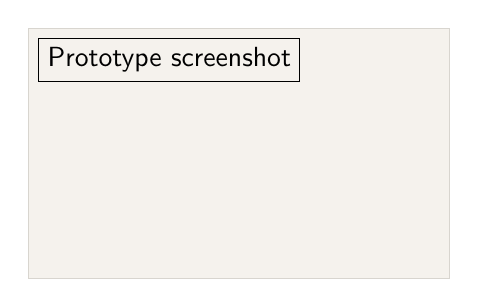
\begin{tikzpicture}
        \begin{scope}
        \clip (0,0) rectangle (5.35,3.18);
        \fill[Pale] (0,0) rectangle (5.35,3.18);
        \node[anchor=north west,inner sep=0] at (.12,3.06)
          {\IfFileExists{assets/demo_baseline.png}{\includegraphics[width=5.10cm]{assets/demo_baseline.png}}{\fbox{Prototype screenshot}}};
        \end{scope}
        \draw[Rule] (0,0) rectangle (5.35,3.18);
      \end{tikzpicture}
      \smallnote{The prototype runs now. Slide 8 shows the full view.}
    \end{column}
  \end{columns}
  \vfill
  \smallnote{Prepared by \TeamName\quad \textperiodcentered{} \University\quad \textperiodcentered{} October 2026}
\end{frame}

% 2. INTRO / TEAM
\begin{frame}{Who we are and what we built}
  \begin{columns}[T,totalwidth=\linewidth]
    \begin{column}{.50\linewidth}
      \kicker{Student team}
      \begin{tabular}{@{}p{1.75cm}p{4.7cm}@{}}
        \MemberOne & Data cleaning and checks \\[.20cm]
        \MemberTwo & Models and validation \\[.20cm]
        \MemberThree & Interface and demo \\
      \end{tabular}
      \vspace{.55cm}
      \smallnote{Replace these names, these roles and the university before you submit.}
    \end{column}
    \begin{column}{.46\linewidth}
      \kicker{Current status}
      \begin{itemize}\setlength\itemsep{.27cm}
        \item Our two notebooks run from start to end.
        \item We compared five readable models on a forward time split.
        \item The simulator is one HTML file. It runs with no server.
        \item The browser sliders and Python give the same numbers.
      \end{itemize}
    \end{column}
  \end{columns}
  \vfill
  {\color{Rule}\rule{\linewidth}{.5pt}}\par
  \smallnote{We want a first tool that a planner can question. We do not want a forecast that nobody can explain.}
\end{frame}

% 3. PROBLEM
\begin{frame}{The planning question}
  \kicker{Why this matters}
  \begin{columns}[T,totalwidth=\linewidth]
    \begin{column}{.54\linewidth}
      {\fontsize{21}{24}\selectfont\bfseries If flights change, what happens to hotel demand?}\par\vspace{.20cm}
      Airlines and hotels plan from different files. One seat can hold a transfer passenger, a returning resident or a hotel guest. So a direct seat-to-room number would be wrong.
    \end{column}
    \begin{column}{.42\linewidth}
      \kicker{Questions to test}
      \begin{itemize}\setlength\itemsep{.16cm}
        \item What if the flights per week go up or down?
        \item What if an airline uses a larger aircraft?
        \item Which months and markets moved most in the past data?
      \end{itemize}
    \end{column}
  \end{columns}
  \vfill
  {\color{Accent}\rule{.07cm}{.45cm}}\hspace{.15cm}%
  \smallnote{The challenge asks for a tool that works, shows its steps and has a back-test. Source: ATP 2026 DCT Abu Dhabi challenge statement.}
\end{frame}

% 4. DATA AND ASSUMPTIONS
\begin{frame}{The two files count countries differently}
  \begin{columns}[T,totalwidth=\linewidth]
    \begin{column}{.46\linewidth}
      \kicker{What the files contain}
      \begin{itemize}\setlength\itemsep{.14cm}
        \item The flight file gives daily seats, passengers and connections.
        \item The hotel file gives daily \emph{Guests} by nationality.
        \item The hotel file has 45 nationalities. 33 match a flight origin by name.
        \item The \emph{Guests} numbers stop in July 2025.
      \end{itemize}
    \end{column}
    \begin{column}{.50\linewidth}
      \kicker{Our stated assumptions}
      \begin{itemize}\setlength\itemsep{.14cm}
        \item We link an origin to a nationality by name. This is an assumption, not a measurement.
        \item The other 12 nationalities get a calendar forecast. Their flight sliders stay off.
        \item We call the monthly sum of \emph{Guests} reported guest-days. We cannot separate capture, length of stay and occupancy.
      \end{itemize}
    \end{column}
  \end{columns}
  \vspace{.18cm}
  \smallnote{We drop the days with no hotel number. We start in 2023 because the 2022 flight rows are monthly, not daily.}
\end{frame}

% 5. SYSTEM DESIGN
\begin{frame}{How the simulator works}
  \kicker{First plain arithmetic, then a fitted response}
  \begin{center}
  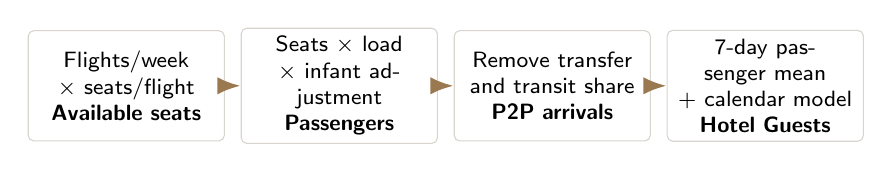
\begin{tikzpicture}[node distance=.20cm,>=Latex,
    box/.style={draw=Rule,fill=white,rounded corners=2pt,align=center,minimum height=1.40cm,text width=2.28cm,inner sep=3pt,font=\footnotesize},
    arr/.style={->,very thick,color=Accent}]
    \node[box] (a) {Flights/week\\$\times$ seats/flight\\\strong{Available seats}};
    \node[box,right=of a] (b) {Seats $\times$ load\\$\times$ infant adjustment\\\strong{Passengers}};
    \node[box,right=of b] (c) {Remove transfer\\and transit share\\\strong{P2P arrivals}};
    \node[box,right=of c] (d) {7-day passenger mean\\+ calendar model\\\strong{Hotel Guests}};
    \draw[arr] (a)--(b); \draw[arr] (b)--(c); \draw[arr] (c)--(d);
  \end{tikzpicture}
  \end{center}
  \vspace{.08cm}
  \begin{columns}[T,totalwidth=\linewidth]
    \begin{column}{.48\linewidth}
      \kicker{Inputs}
      Market, month, flights per week, seats per flight, load factor and transfer/transit share.
    \end{column}
    \begin{column}{.48\linewidth}
      \kicker{Outputs}
      Predicted guest-days, the change from the real flights, the daily profile, the learned response and a warning for extreme inputs.
    \end{column}
  \end{columns}
  \vfill
  \smallnote{The fitted response holds the step from visitor to hotel guest. We cannot measure that step on its own.}
\end{frame}

% 6. MODEL
\begin{frame}{We chose the simpler model on evidence}
  \begin{columns}[T,totalwidth=\linewidth]
    \begin{column}{.50\linewidth}
      \kicker{Five candidates}
      \begin{enumerate}\setlength\itemsep{.14cm}
        \item Calendar-only baseline
        \item Proportional passenger chain
        \item Monotonic regression \strong{(selected)}
        \item Monotonic GAM, 7-day exposure
        \item Monotonic GAM, stay-kernel exposure
      \end{enumerate}
      \vspace{.2cm}
      \smallnote{The two GAMs scored a little worse on the selection months. The extra curve gave no gain, so we left it out.}
    \end{column}
    \begin{column}{.46\linewidth}
      \kicker{Readable response}
      \begin{center}
      \colorbox{Pale}{\parbox{.94\linewidth}{\centering\vspace{.15cm}
        $\log(1+\widehat{G})=\alpha_{m}+\beta_{m}\log(1+P_{7})$\\[.08cm]
        $+\;\text{month}+\text{weekday}+\text{trend}$\\[.08cm]
        $\beta_{m}\geq 0$\vspace{.15cm}}}
      \end{center}
      Each matched market gets one coefficient. The coefficient cannot go below zero, so more passengers never lower demand. The seven-day mean lets an effect build up over days.
    \end{column}
  \end{columns}
  \vfill
  \smallnote{We chose the model on Jan--Apr 2025 only. If two models are within 1 point, we take the simpler one.}
\end{frame}

% 7. VALIDATION
\begin{frame}{What the back-test shows}
  \kicker{Lower WMAPE is better}
  \begin{columns}[T,totalwidth=\linewidth]
    \begin{column}{.51\linewidth}
      \small
      \begin{tabular}{@{}p{3.2cm}rr@{}}
        \toprule
        & Calendar & Flight model \\
        \midrule
        Jan--Apr 2025 selection & 31.9\% & \strong{25.0\%} \\[.15cm]
        Jun--Jul 2025 audit & 35.0\% & \strong{27.7\%} \\
        \bottomrule
      \end{tabular}
      \vspace{.28cm}
      \smallnote{WMAPE $=\sum|\text{prediction}-\text{observed}|/\sum\text{observed}$ over all nationality-days. We fit the models on Jan 2023--Dec 2024 after a 27-day warm-up. We keep May 2025 for the error bands.}
    \end{column}
    \begin{column}{.45\linewidth}
      \kicker{Our reading}
      \stat{7.2 points}{Less error on the months we held back.}
      \vspace{.42cm}
      \stat{27.7\%}{Still too much error for one market on its own.}
    \end{column}
  \end{columns}
  \vfill
  \smallnote{The daily total error is 6.5\%, because one market's error can cancel another's. The test uses the flights that did operate. We changed no flights.}
\end{frame}

% 8. MOCK-UP / PROTOTYPE
\begin{frame}{A working prototype, not just a diagram}
  \begin{columns}[T,totalwidth=\linewidth]
    \begin{column}{.53\linewidth}
      \kicker{What a planner can do now}
      \begin{enumerate}\setlength\itemsep{.17cm}
        \item Pick a market and a month.
        \item Move one slider: flights per week, seats per flight, load factor or connecting share.
        \item Compare your scenario with the real flights. Read the passenger steps and the demand curve.
        \item Watch for the warning when the scenario goes past the training range.
      \end{enumerate}
      \vspace{.25cm}
      \smallnote{The prototype is one HTML file and needs no network. We check the browser math against Python.}
    \end{column}
    \begin{column}{.43\linewidth}
      \centering
      \IfFileExists{assets/demo_baseline.png}{%
        \fbox{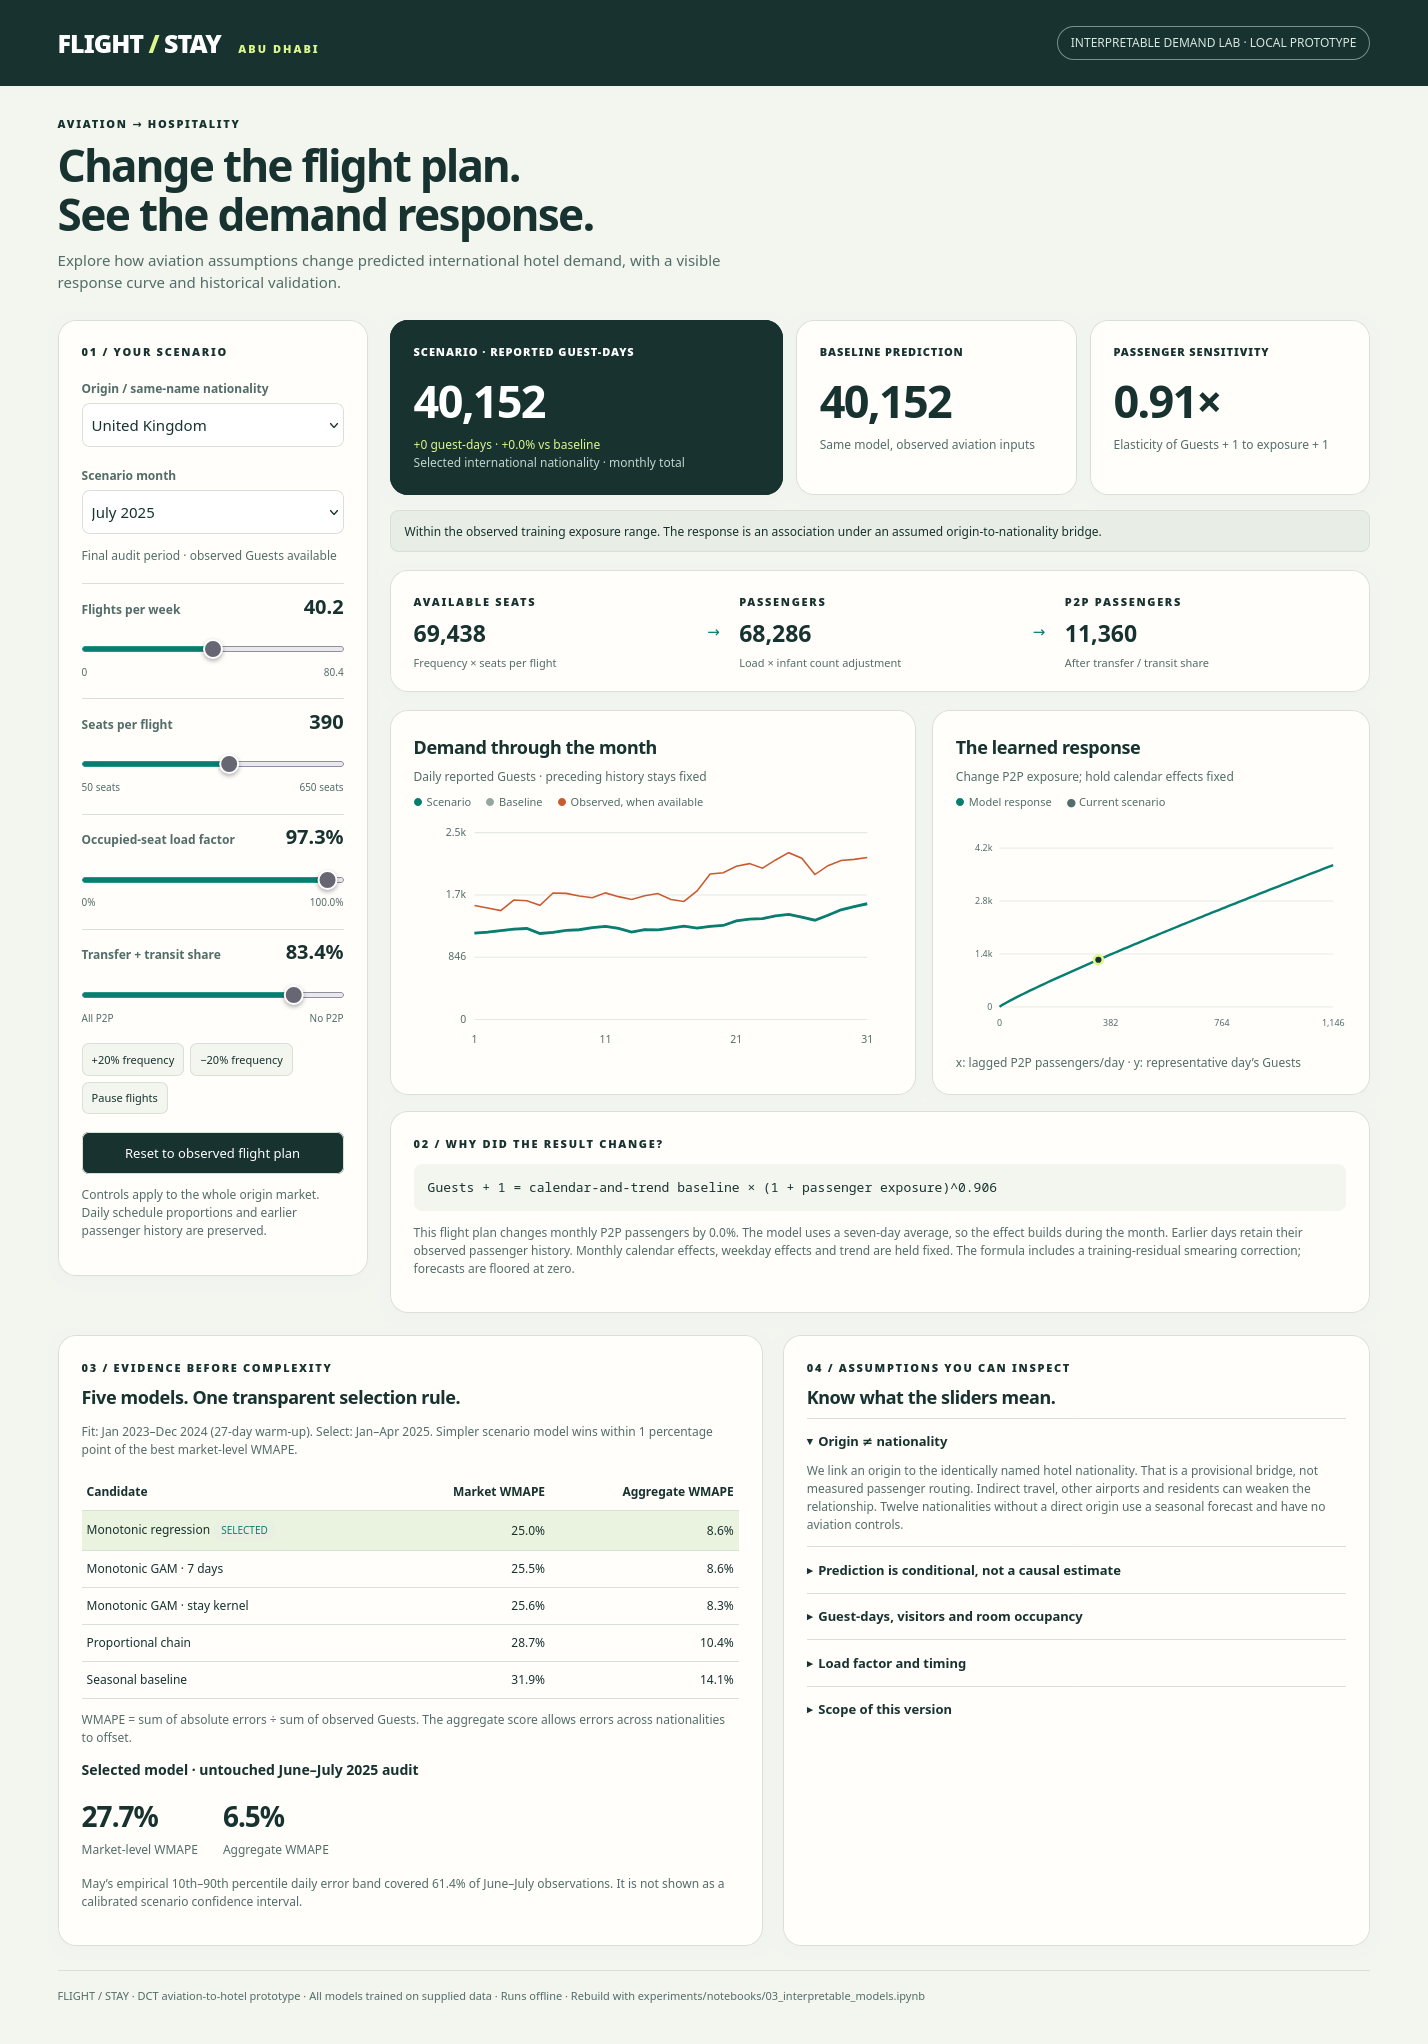
\includegraphics[height=5.65cm]{assets/demo_baseline.png}}%
      }{\fbox{\parbox[c][5.4cm][c]{5cm}{\centering Screenshot: prototype with four sliders and prediction cards}}}
      \par\smallnote{The HTML prototype, UK / July 2025.}
    \end{column}
  \end{columns}
\end{frame}

% 9. IMPACT AND FEASIBILITY
\begin{frame}{Where this could be useful}
  \begin{columns}[T,totalwidth=\linewidth]
    \begin{column}{.47\linewidth}
      \kicker{Intended impact}
      \begin{itemize}\setlength\itemsep{.16cm}
        \item Show the flight and hotel assumptions in one place.
        \item Compare scenarios for current markets before a deeper study.
        \item Point to the months and markets that react most, for a person to review.
      \end{itemize}
    \end{column}
    \begin{column}{.49\linewidth}
      \kicker{Real-life requirements}
      \begin{itemize}\setlength\itemsep{.16cm}
        \item Ask DCT what \emph{Guests} counts. Ask for room counts, so we can show occupancy.
        \item Improve the link from flight origin to nationality with approved aggregate data.
        \item Reload the source data often. Track the error by market and by season.
        \item Keep new routes switched off until we can support them with evidence.
      \end{itemize}
    \end{column}
  \end{columns}
  \vfill
  {\color{Rule}\rule{\linewidth}{.5pt}}\par
  \smallnote{Today the slider shows an association under the assumptions above. It is not a proven effect of adding flights.}
\end{frame}

% 10. SHORTLIST TEST PLAN + SOURCES
\begin{frame}{If shortlisted: test the hard part}
  \begin{columns}[T,totalwidth=\linewidth]
    \begin{column}{.57\linewidth}
      \kicker{Demo and test plan}
      \begin{enumerate}\setlength\itemsep{.12cm}
        \item Show three runs for one market and month: the baseline, 20\% more flights, and a route cut.
        \item Ask DCT to state the target definitions and the origin-to-nationality map.
        \item Name the new test months and the real route changes first. Then check the error and the direction of the change.
        \item Report the misses by market, by season and by how far the scenario goes past the data. Change the model only against months we have not used.
      \end{enumerate}
    \end{column}
    \begin{column}{.39\linewidth}
      \kicker{What we need to improve}
      We need aggregate origin--nationality flows, a guest-night definition from DCT, event dates and room counts. With those we could test more of the seats-to-visitors-to-nights chain.

      \vspace{.40cm}
      \smallnote{The prototype and the notebooks are ready for a live demo. Add the team details and the video link before you submit.}
    \end{column}
  \end{columns}
  \vfill
  {\color{Rule}\rule{\linewidth}{.5pt}}\par
  \tiny Sources: the ATP 2026 DCT Abu Dhabi challenge statement (challengeon.atrc.ae). The supplied DCT aviation and hotel files. Our domain analysis and model-comparison notebooks. We reproduced the results on 11 October 2026.
\end{frame}

\end{document}
